
\part*{Kinetik}


\section*{Orts-, Geschwindigkeits- und Beschleunigungsfunktionen}


\subsection*{Ortsfunktion}
\begin{verse}
$\vec{r}(t)=\left(\begin{array}{c}
x(t)\\
y(t)\\
z(t)
\end{array}\right)$
\end{verse}

\subsubsection*{Geschwindigkeit}

Die Geschwindigkeit ist die zeitliche Ableitung der Ortsfunktion:
\begin{verse}
$\vec{v}(t)=\frac{d\vec{r}(t)}{dt}=\vec{r'}(t)=\left(\begin{array}{c}
\frac{dx(t)}{dt}\\
\frac{dy(t)}{dt}\\
\frac{dz(t)}{dt}
\end{array}\right)=\left(\begin{array}{c}
x'(t)\\
y'(t)\\
z'(t)
\end{array}\right)=\left(\begin{array}{c}
v_{x}(t)\\
v_{y}(t)\\
v_{z}(t)
\end{array}\right)$
\end{verse}
Geschwindigkeit ist ein Vektor, die Schnelligkeit ihr Betrag.


\subsection*{Beschleunigung}

Die Beschleunigung ist die zeitliche Ableitung der Geschwindigkeits
resp. die zweite zeitliche Ableitung der Ortsfunktion.
\begin{verse}
$\vec{a}(t)=\frac{d\vec{v}(t)}{dt}=\left(\begin{array}{c}
\frac{dv_{x}(t)}{dt}\\
\frac{dv_{y}(t)}{dt}\\
\frac{dv_{z}(t)}{dt}
\end{array}\right)\left(\begin{array}{c}
a_{x}(t)\\
a_{y}(t)\\
a_{z}(t)
\end{array}\right)$

$\vec{a}(t)=\frac{d}{dt}\left(\frac{d\vec{r}(t)}{dt}\right)=\frac{d^{2}\vec{r}(t)}{dt^{2}}$
\end{verse}
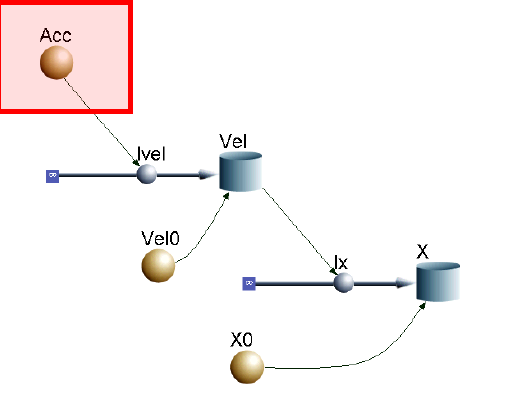
\includegraphics[scale=0.6]{Kinetik/BM}


\section*{Kraft}

Die Kraft ist das Produkt von Masse und Beschleunigung:
\begin{verse}
$\vec{F}=m\cdot\vec{a}$

$\left[\vec{F}\right]=\left[\frac{kg\cdot m}{s^{2}}\right]=\left[N\right]$
\end{verse}

\section*{Schiefer Wurf}
\begin{verse}
$\vec{a}=\left(\begin{array}{c}
0\\
0\\
-g
\end{array}\right)\Rightarrow\vec{v}=\left(\begin{array}{c}
v_{x0}\\
v_{y0}\\
v_{z0}-gt
\end{array}\right)\Rightarrow\vec{r}=\left(\begin{array}{c}
r_{x0}+v_{x0}\\
r_{y0}+v_{y0}\\
r_{z0}+v_{z0}-g\frac{t^{2}}{2}
\end{array}\right)$
\end{verse}

\section*{Kreisbewegung}

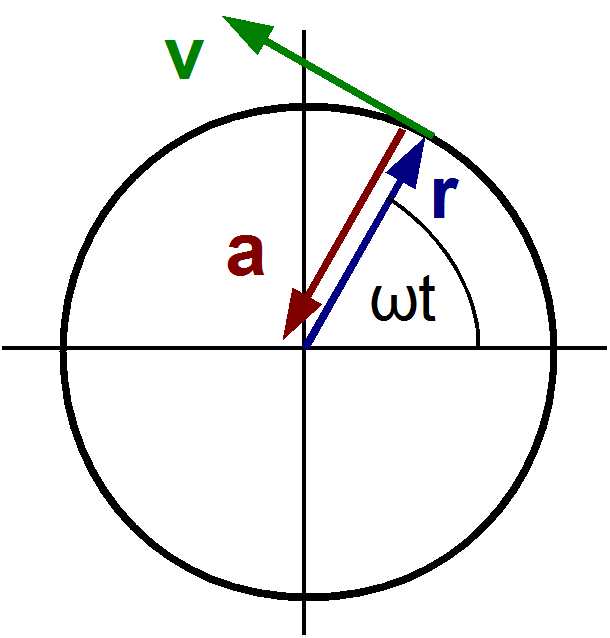
\includegraphics[height=6cm]{Kinetik/Kreisbewegung}
\begin{verse}
$\omega$ = Winkel pro Sekunde

$T=\frac{2\Pi}{\omega}=$Periode, Zeit für einen Umlauf ($360^{\circ}=2\Pi$)
\end{verse}

\subsection*{Ortsvektor}
\begin{verse}
$\vec{r}(t)=\left(\begin{array}{c}
r\, cos(\omega t)\\
r\, sin(\omega t)
\end{array}\right)$

$|\vec{r}(t)|=r$

$\vec{r}(t)=\left(\begin{array}{c}
r\, cos(\omega(t+T))\\
r\, sin(\omega(t+T))
\end{array}\right)=\left(\begin{array}{c}
r\, cos(\omega t+2\Pi)\\
r\, sin(\omega t+2\Pi)
\end{array}\right)=\left(\begin{array}{c}
r\, cos(\omega t)\\
r\, sin(\omega t)
\end{array}\right)$
\end{verse}

\subsection*{Geschwindigkeit}
\begin{verse}
$\vec{v}(t)=\frac{d\vec{r}(t)}{dt}=\left(\begin{array}{c}
-r\omega sin(\omega t)\\
r\omega cos(\omega t)
\end{array}\right)$

$|\vec{v}(t)|=r\omega$
\end{verse}

\subsection*{Beschleunigung}
\begin{verse}
$\vec{a}(t)=\frac{d\vec{v}(t)}{dt}=\left(\begin{array}{c}
-r\omega^{2}cos(\omega t)\\
-r\omega^{2}sind(\omega t)
\end{array}\right)$

$|\vec{a}(t)|=r\omega^{2}$\end{verse}

